\documentclass[conference,onecolumn]{IEEEtran}
\usepackage{hyperref}
\usepackage[utf8]{inputenc}
\usepackage[french]{babel}
\usepackage{amsmath,amssymb,amsfonts}
\usepackage{mathtools}
\usepackage{algorithmic}
\usepackage{graphicx}
\usepackage{textcomp}
\usepackage{xcolor}
\usepackage{float}
\usepackage{lipsum, babel}
\usepackage[T1]{fontenc}
\def\BibTeX{{\rm B\kern-.05em{\sc i\kern-.025em b}\kern-.08em
    T\kern-.1667em\lower.7ex\hbox{E}\kern-.125emX}}
    

% Inicio del documento
\begin{document}

\title{Atténuation du bruit dans des signaux audios a travers l’implémentation de méthodes classiques et une méthode hybride\\
}

\author{\IEEEauthorblockN{1\textsuperscript{st} José Miguel Galindo Barco}
\IEEEauthorblockA{\textit{Ecole d’ingénieurs}\\
\textit{Génie de systèmes} \\
\textit{Université EAFIT}\\
\href{mailto:jmgalindob@eafit.edu.co}{jmgalindob@eafit.edu.co}
}
\and
\IEEEauthorblockN{2\textsuperscript{nd} Juan José Tamayo Acevedo}
\IEEEauthorblockA{\textit{Ecole de sciences}\\
\textit{Génie mathématique} \\
\textit{Université EAFIT}\\
\href{mailto:jjtamayoa@eafit.edu.co}{jjtamayoa@eafit.edu.co}
}
\and
\IEEEauthorblockN{3\textsuperscript{rd} Salomón Cardeño Luján}
\IEEEauthorblockA{\textit{Ecole de sciences}\\
\textit{Génie mathématique} \\
\textit{Université EAFIT}\\
\href{mailto:scardenol@eafit.edu.co}{scardenol@eafit.edu.co}
}
}

\maketitle

\begin{abstract}
L’atténuation du bruit est un domaine d’étude actif dans des milieux comme le traitement digital et analogique des signaux. Dans ce domaine il existe une grande variété d’algorithmes et/ou méthodes classiques et modernes qui sont utilisé dans ce but. Dans ce travail de recherche, nous réaliserons une étude théorique du filtre analogique passe-bas avec une approximation de Butterworth, le filtre de Weiner et la méthode dite hybride de DSP/Deep Learning RNNbruit. Puis nous développerons une analyse de ces trois méthodes où nous comparerons les résultats de signaux lorsque nous filtrons un signal propre, un signal avec addition de bruit blanc, un signal avec addition de bruit rosa et un signal avec addition de bruit rouge. Les enregistrement audios résultant de chaque méthode filtrage seront comparer qualitativement et quantitativement, d’où la nécessité de tenir en compte la perception auditive du récepteur. Finalement, nous proposerons des modifications sur la mise en œuvre ou implémentation de ces méthodes en considérant le contexte et le bon fonctionnement dans ce dernier. 
\end{abstract}

\section{Introduction}
HAY QUE PONER ALGO AQUÍ

\section{Concepts fondamentaux}

\begin{itemize} % Lista
    \item[] \textbf{Signal}: un signal est la representation physique de l'information, qu'il convoit de sa source a sa destination.

    \item[] \textbf{Bruit}: Un bruit correspond a tout phénomène gênant la transmission ou l'interpretation d'un signal

    \item[] \textbf{Traitement du signal}: Le traitement du signal est une discipline qui étudie des méthodes de traitement, d’analyse et d’interprétation des signaux. Pour cela, dans ce domaine on utilise des méthodes tels que le contrôle, le filtrage, la compression et la transmission de données, la réduction du bruit, la déconvolution, la prédiction, l'identification, la classification.  

    \item[] \textbf{Filtrage}: On appelle "filtrage" toute application qui, à un signal $f_e(t)$, dit "signal d'entrée", associe un signal $f_s(t)$, dit "signal de sortie", tel que le module du spectre de $f_s(t)$ soit inférieur ou égal au module du spectre de $f_s(t)$, pour w réel quelconque. 
\end{itemize}

\subsection{Signal sonore et note audio}
Le son ou signal sonore est une perturbation mécanique d’un état d’équilibre, qui se propage à travers d’un milieu solide élastique. Il est possible de le définir subjectivement comme ceux qui est perçu par l’ouïe, mais cela reviendra à restreindre la définition même d’un signal. De même, la lumière est perçue par la vue mais il existe certaines longueurs d’ondes lumineuse qui ne sont pas perçu par l’œil humain. Il existe donc des domaines de fréquences des signaux sonores qui ne sont pas perçu par l’ouïe humain. 

Dans un premier temps, en s’appuyant sur le point de vue physique, les ondes sonores se propage à travers l’air ou autres milieux (solides et élastiques) sous forme de longueur d’ondes, où la vibration mécanique qui décrit l’onde se propage dans la même direction que la propagation de celle-ci. L’air peut être compris comme un milieu élastique sur lequel les particules, ou tout simplement les couches d’air, ont un comportement semblable à un ressort, c’est-à-dire qu’elles “se poussent” et “s’attirent” les unes avec les autres. 

Plus clairement, une onde sonore est une variation periodique ou sinusoidale de la pression d’un milieu pendant un temps precis dans un endroit precis. 

Dans la figure ci-dessous, dans un premier temps nous pouvons voir l’air dans son equilibre (figure xA), le variations dans l’air lorsqu’une onde sonore pure se deplace dans ce milieux (figure xB) et l’allure de  l’onde qui se déplace dans l’air.

% Imagen
\begin{figure}[H]
 \centering
    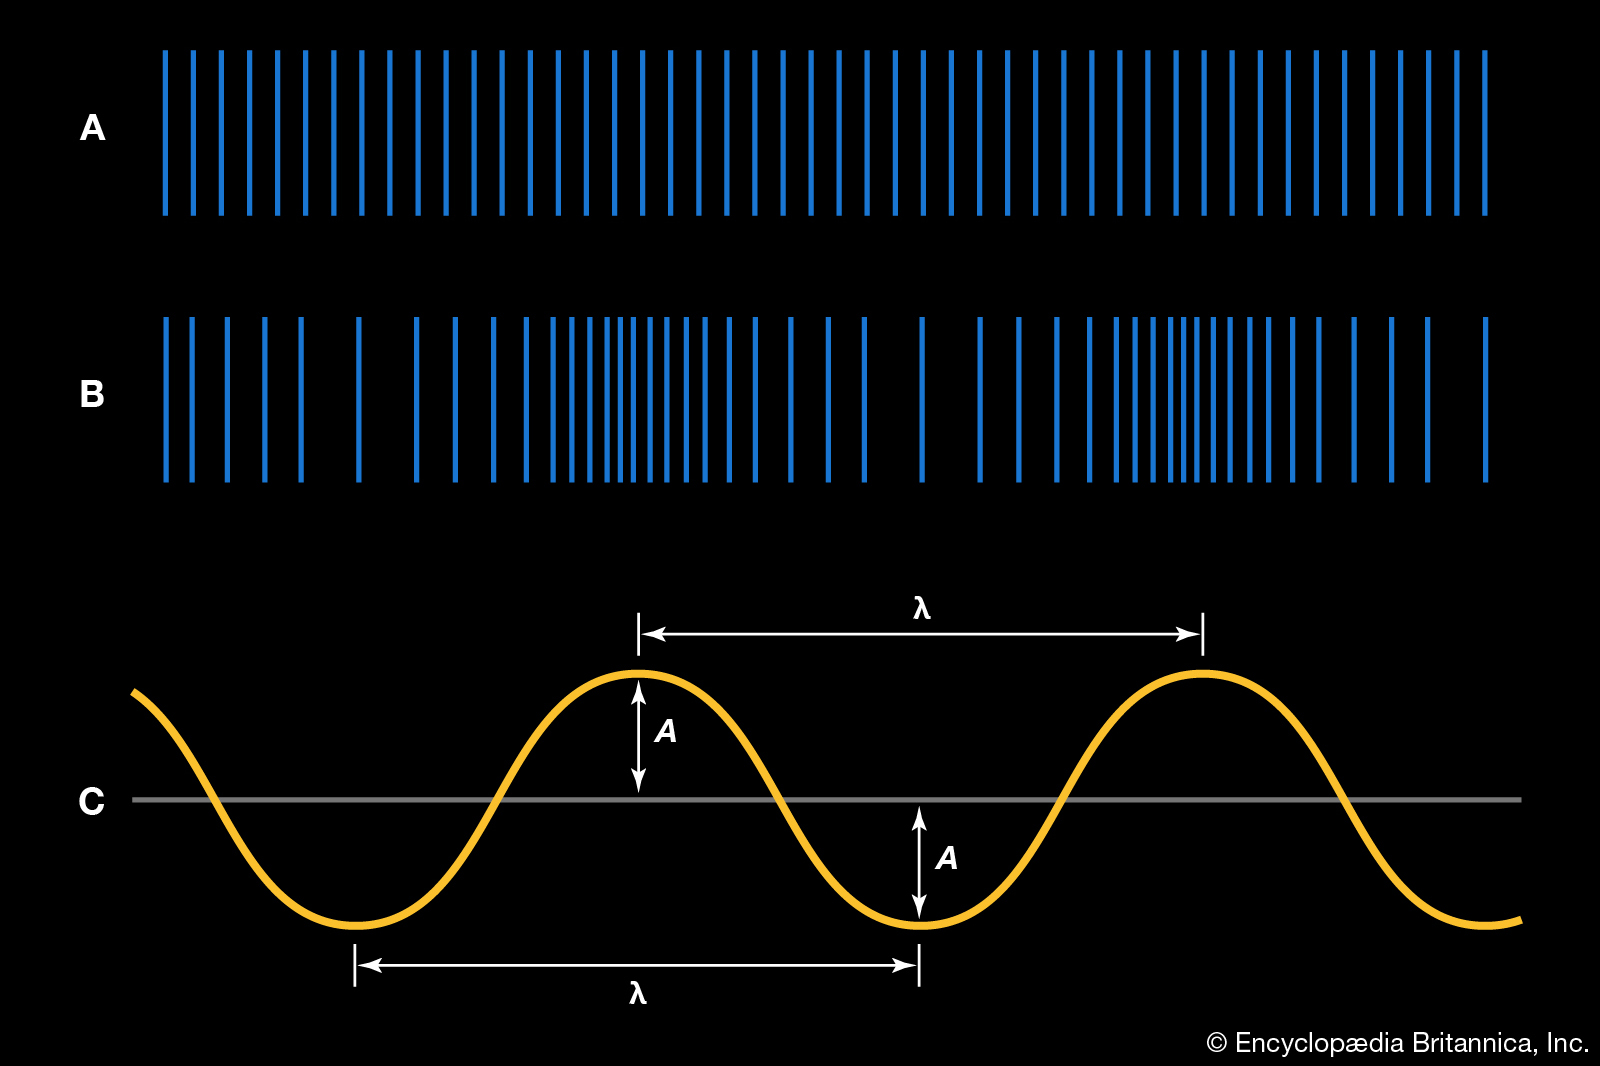
\includegraphics[scale=0.2]{img1.jpg}
    \caption{Représentations graphiques d’une onde sonore. (A) L’air à l’équilibre, avec l’absence de l’onde sonore. (B) compressions et réfractions qui constituent l’onde sonore. (C) Représentation graphique de l’onde sonore avec son amplitude A et sa longueur d’onde $\lambda$.}
\end{figure}

\subsection{Caractéristiques physique et description mathématique d’un signal sonore }

Il est important de remarque que dans figure précédente, plus précisément dans la partie C de cette figure, s’agit d’une autre représentation du signal sonore illustré dans la partie B. En effet, dans cette partie nous pouvons voire une courbe sinusoïdale, cette courbe représente la variation de la pression du signal sonore, celui-ci se répète de façon périodique. La distance entre 2 pics de la courbe est nommée longueur d’onde et se représente par la lettre $\lambda$. 

Lorsqu’un signal sonore ou onde sonore se déplace dans l’air, la longueur d’onde prend un certain temps pour aller d’un point $A$ à un point $B$ de l’espace, cette durée de temps est appelée période et note T. 

De plus, pendant un intervalle de temps équivalent à une seconde, un certain nombre de longueurs d’onde passe d’un point A à un point de l’espace. Ce phénomène est connu comme fréquence du signal. Dans d’autres mots, la fréquence est le nombre de périodes par unité de temps ce qui correspond à l’inverse de la période : $f=1/T$ ou f est la fréquence en Hertz ($Hz$ ou $s^-1$) et $T$ la période en seconde ($s$). 

Il est important de remarquer que les signaux sonores qui ont de hautes fréquences, ont des périodes courtes, alors que les signaux sonores qui ont des bases fréquences, ont de longs périodes. De plus, l’intervalle de fréquences que l’être humain peut percevoir se trouve entre les $20Hz$ et les $20 kHz$. Il existe une propriété physique qui permet de classifier les signaux sonores en fonction de la perception physiologique des êtres humains, cette propriété est connue comme le ton. En plus, les signaux ont une vitesse de déplacement, celle-ci est connue comme vitesse de l’onde ($S$), elle est obtenue par une relation entre la fréquence ou la période et la longueur d’onde, comme montrer ci-dessous : 

\[S = f*\lambda = \dfrac{\lambda}{T}\]

Le déplacement d’une onde sonore dans une dimension (signal sonore plat) est décrit mathématiquement par l’équation général du mouvement des ondes, qui peut être écrit de la façon suivante :  
 
\[y(x,t) = Asin(2\pi(ft - \dfrac{x}{\lambda}))\]

L'amplitude ($A$) d'une onde correspond à la hauteur maximale atteinte par l'onde par rapport à sa position n au repos. 

De plus, grâce à l’amplitude nous pouvons déterminer intensité de l’onde, qui est perçu par l’ouïe sous le nom de volume. L'intensité acoustique ($I$), est définie comme le taux de transmission d'énergie par unité d’aire perpendiculaire à la direction de propagation de l’onde. La relation existante entre l’intensité et l’amplitude est la suivante : 

\[I = \dfrac{A^2}{2\rho S}\]

Avec :

\begin{itemize} % Lista

    \item[-] $\rho$ : densité de l’air à l’équilibre (en $kg/m^3$).
    \item[-] $S$ vitesse de l’onde (en $m/s$).

\end{itemize}

L’intensité $I$ a pour unité les watt par mètre carré ($W/m^2$). Sous des “conditions atmosphériques standards, on a : 

\[\rho=10^5 Pa=10^5 \dfrac{N}{m^2}\]

L’amplitude minimum de variation de pression que l’ouïe humain peut percevoir es de $10^-5 Pa$ et l’amplitude maximal est de $10 Pa$. 

\subsection{Audition et perception du son chez les êtres humains}

D’après ce qui a été décrit précédemment, il est convenable de remarque les faits suivants :

\begin{itemize} % Lista

    \item[-] Entre $20 Hz et 20 kHz$ se trouve l’intervalle de fréquence perçu par l’être humain.  

    \item[-] L’amplitude d’une onde sonore permet de déterminer l’intensité de l’onde. 

    \item[-] L’amplitude minimum de variation de pression que l’ouïe humain peut percevoir es de $10^-5 Pa$ et l’amplitude maximal est de $10 Pa$.

\end{itemize}

\subsection{Echelles des décibels}

L’échelle des décibels est une échelle qui permet de classifie les ondes sonores en fonction de leur intensité sonore. Cette échelle est décrite par l’équation suivante : 

\[I_{dB} = L = 10log(\dfrac{I}{I_0})\]

Avec L qui représente les décibels, $I$ l’intensité de l’onde et $I_0=10^{-12}$ $W/m^2$ es l’intensité de référence. 

Plus précisément, L’échelle des décibels est logarithmique, ce qui signifie qu’une augmentation du niveau sonore de $3 dB$ représente déjà un doublement de l’intensité sonore. Par exemple, le volume d’une conversation normale peut être d’environ $65 dB$ et, pour quelqu’un qui crie, ce chiffre peut atteindre environ $80 dB$. La différence est seulement de $15 dB$, mais le cri représente une intensité trente fois supérieure. 

Le décibel ($dB$) est une unité utilisée pour mesurer l'intensité des sons et celle d'autres grandeurs physiques. Un décibel équivaut à un dixième de bel ($B$), une unité qui doit son nom à Graham Bell, l'inventeur du téléphone. Son échelle logarithmique permet de représenter le spectre auditif de l’être humain dans son ensemble.

% Imagen
\begin{figure}[H]
 \centering
    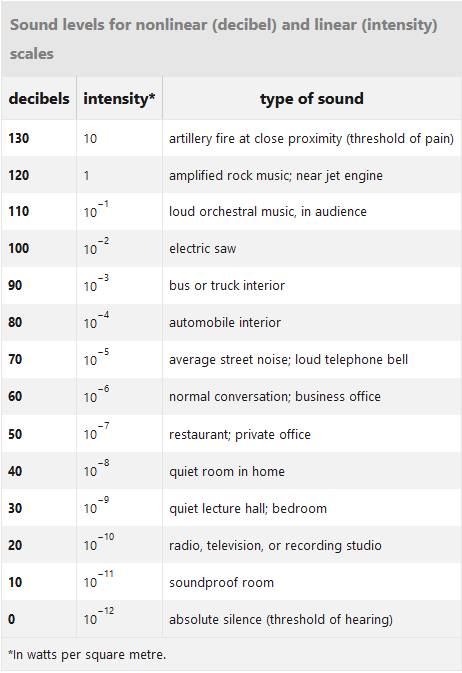
\includegraphics[scale=0.6]{img2.png}
\end{figure}

 Le champ auditif de l’être humain (en vert) est limité par une courbe qui nous fournis la limite inferieur et une autre courbe qui nous donne la limite supérieure de la perception sonore. A caque fréquence, entre $20 Hz et 20 kHz$, le seuil de notre sensibilité est différent. L’intervalle le plus large de perception a lieu aux alentours les $2 kHz$ et commence à partir des $0 dB$. Dans cet intervalle dit “moyen” les dynamiques sensorielles sont les plus aptes possibles et peuvent avoir un équivalent de $130 dB$.
 
% Imagen
 \begin{figure}[H]
 \centering
    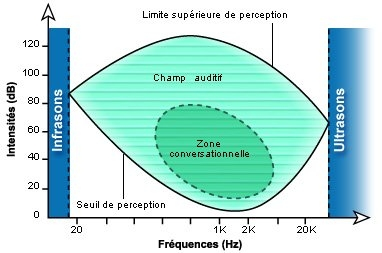
\includegraphics[scale=1.5]{img3.jpg}
    \caption{Courbe audiométrique de l'oreille humaine.}
\end{figure}

 \subsection{Tonalité pure}
 Lorsque nous utilisant de fonction comme celle de la vitesse de déplacement d’une onde, nous pouvons dire que cette fonction représente une tonalité pure avec un fréquence $f$. Ce nom dérive du fait que cette fonction décrit une onde sonore avec une seule composante en fréquence, c’est-à-dire qu’il s’agit d’un cas idéal, parce que en faisant analogie avec la lumière, dans la nature nous ne trouverons jamais une lumière monochromatique (d’une seule couleur, c’est-à-dire d’une seule fréquence), nous ne trouverons jamais une onde sonore avec cette caractéristique.  

Afin de donner une définition plus précise d’une tonalité pure, nous devons nous appuyer sur la définition donnée en psychoacoustique. En effet, en psychoacoustique, une tonalité pure, ou encore son pur ou note pure (en anglais : pure tone) est un son avec une forme d'onde sinusoïdale ; c'est-à-dire une onde sinusoïdale de n'importe quelle fréquence, phase et amplitude. En audiologie clinique, les tons purs sont utilisés pour l'audiométrie tonale (en) afin de caractériser les seuils d'audition à différentes fréquences. 

\subsection{Descomposición del sonido en tonos puros}
Proprement dit, toute onde sonore resulte de l’addtion de plusieurs tonalité pure de frequence differente. La quantite de 

Formalmente, cualquier sonido $f$ es una suma de tonos puros a diferentes frecuencias. La cantidad de cada frecuencia requerida para formar el sonido $f$ es el contenido frecuencial de $f$. Cualquier sonido puede ser reconstruido partiendo de su contenido frecuencial.

Una implicación de lo anterior es que, en general, cualquier sonido puede ser considerado como una función, y por más complejo que sea el sonido, puede ser representado por la suma de tonos puros o funciones sinusoidales (senos y cosenos) lo cual no es sorpresa que esté relacionado con el concepto matemático de series de Fourier. 

Adicionalmente, lo anterior también implica que el sonido $f$ puede ser almacenado al guardar simplemente su contenido frecuencial, como una alternativa de guardar a $f$ como tal.

\subsection{Espectro del sonido}
El espectro del sonido muestra las diferentes frecuencias presentes en un sonido, es decir, muestra el contenido frecuencial que caracteriza el sonido en particular y con qué amplitud está presente, respectivamente. Usualmente es presentado como una gráfica de frecuencia versus intensidad, presión o potencia en $dB$. Cabe aclarar que si es evidente que hay una frecuencia dominante (de mayor amplitud) se le llama frecuencia fundamental y al resto armónicos. A continuación observe el ejemplo de una flauta que toca la nota G4 equivalente a aproximadamente $400 Hz$ ; note que esta es la frecuencia fundamental o predominante con mayor amplitud y el resto son sus armónicos. Si se comparara esta misma nota en otro instrumento también se obtendría la misma frecuencia predominante, pero sus armónicos serían distintos y esto es lo que hace que los seres humanos percibamos cada instrumento de forma distinta aún tocando la misma nota. Esta percepción auditiva se conoce como el \underline{timbre}.

% Imagen
 \begin{figure}[H]
 \centering
    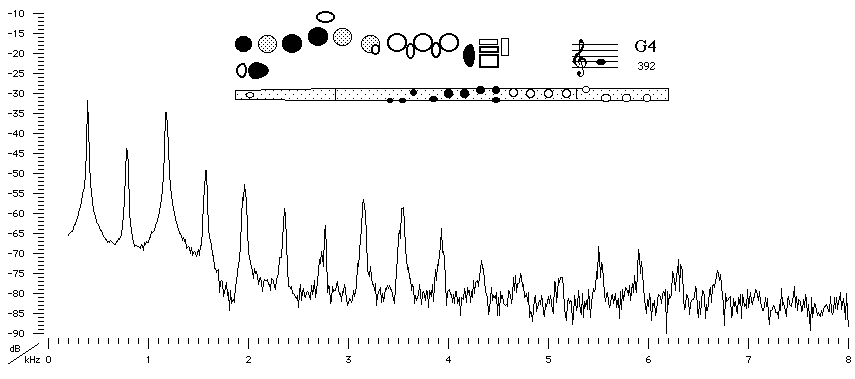
\includegraphics[scale=0.8]{img4.png}
    \caption{Espectro del sonido de una flauta tocando la nota G4 que corresponde aproximadamente a 400Hz. Observe que esta es la frecuencia fundamental y la presencia de armónicos.}
\end{figure}

\subsection{Sonido digital}

L'échantillonnage d'un signal continu est l'opération qui consiste à prélever des échantillons du signal pour obtenir un signal discret, c'est-à-dire une suite de nombres représentant le signal, dans le but de mémoriser, transmettre, ou traiter le signal. 

L'échantillonnage intervient dans l'opération de conversion analogique-numérique, par exemple dans un dispositif de numérisation du son ou de l'image. Un autre exemple d'échantillonnage est celui que l'on fait pour obtenir la représentation graphique d'une fonction à une ou deux variables. D'une manière générale, l'échantillonnage intervient dans toute opération de conversion continu/discret. 

Le théorème de l'échantillonnage de Shannon, qui permet de savoir à quelle fréquence minimale il faut échantillonner un signal pour ne pas perdre l'information qu'il contient. 

Soit $u(t)$ une fonction représentant un signal continu. On considère un échantillonnage périodique défini par : 

où $k$ est un entier. Te est la période d'échantillonnage. $f_e=1/T_e$ est la fréquence d'échantillonnage. 

Le théorème de Shannon ([1]) concerne les signaux dont le spectre possède une fréquence maximale $f_{max}$, que l'on appelle des signaux à bande limitée. Par exemple, si $u(t)$ est un polynôme trigonométrique, la fréquence maximale est celle de la plus grande harmonique.

\textbf{Théorème de Shannon} : pour que le signal puisse être entièrement reconstruit à partir des échantillons, il faut et il suffit que : 

La fréquence d'échantillonnage doit être strictement supérieure à deux fois la plus grande fréquence présente dans le spectre du signal continu (condition de Nyquist-Shannon). Si cette condition est vérifiée alors : 

où la fonction sinus cardinale est définie par : 

Cette relation montre que le signal peut être reconstruit à partir des échantillons, ce qui signifie que toute l'information présente dans le signal original est conservée dans les échantillons. Nous verrons plus loin comment l'opération de reconstruction est effectuée en pratique. 

La moitié de la fréquence d'échantillonnage est appelée la fréquence de Nyquist $f_n$ et la condition de Nyquist-Shannon s'écrit donc $f_{max}<f_n$. 

Lorsque la condition n'est pas vérifiée, on dit qu'il y a sous-échantillonnage. On parle de sur-échantillonnage lorsque la fréquence de Nyquist est beaucoup plus grande que $f_max$. 

Las mediciones normalmente se les conoce como \textit{muestras}. El tiempo entre mediciones sucesivas se le llama \textit{periodo de muestreo} y usualmente es denotado por $T_s$. La longitud del vector usualmente se asume como $N$, e indexado desde $0$ a $N-1$. El proceso de convertir una onda de sonido (audio análogo) a sonido digital se le llama cuantización del audio en donde a cada una de las muestras anteriores se les asocia un valor de amplitud (usualmente entre -$1$ y $1$). El rango de posibles niveles de amplitud, en otras palabras, el número de particiones equiespaciadas del intervalo de valores de amplitud $[-1,1]$ se le conoce como \textit{profundidad de bits}, por ejemplo 

\[8-bit = 2^8 = 256 \quad posibles valores\]
\[16-bit = 2^{16} = 65536 \quad posibles valores\]

Para visualizar el efecto de la cuantización del audio y la influencia de la frecuencia de muestreo y la profundidad de bits observe la figurax a continuación.

% Imagen
 \begin{figure}[H]
 \centering
    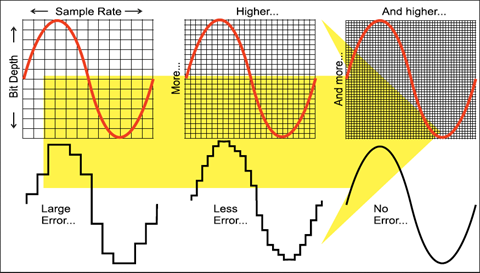
\includegraphics[scale=1]{img5.png}
    \caption{Cuantización de un sonido (audio análogo) y la influencia de la frecuencia de muestreo (Sample Rate) y la profundidad de bit (Bit Depth). Observe que entre mayor sean estos parámetros, mayor será el error cometido en la cuantización.}
\end{figure}

Así como lo sugiere la figura anterior, la frecuencia de muestreo y la profundidad de bit juegan un papel fundamental en la determinación de la calidad del audio resultante.

\subsection{Almacenamiento de un sonido digital en el computador}
En un computador usualmente se utiliza el método de modulación por impulsos codificados (PCM, Pulse-code modulation en inglés) para transformar la señal análoga en una secuencia de bits (señal digital). Este método fue inventado por Alec Reeves en 1937 y es la forma estándar de audio digital en las computadoras. (ref) 

Para que un computador pueda reproducir un sonido digital en el computador las muestras obtenidas deben de ser guardadas en un archivo o en la memoria del computador; en el caso del PCM se almacena en formato RAW o en otros como WAV, AIFF, AU, entre otros. Sin embargo, como los archivos de audio son grandes, lo normal es trabajar con formatos comprimidos que reducen el tamaño del archivo: (ref) \\

\begin{itemize} % Lista

    \item[-] \textbf{Formatos con pérdida} \textit{(lossy)}: son formatos que comprimen el archivo de audio original al eliminar partes de él de acuerdo a un algoritmo de compresión específico, por lo que al descomprimir el archivo no se obtiene el original. Algunos de ellos son : \texttt{MP3, Opus, Vorbis, WMA,} entre otros.
    \item[-] \textbf{Formatos sin pérdida} \textit{(lossless)}: son formatos que comprimen el archivo de audio original al organizar la información de forma eficiente, por lo que al descomprimir el archivo se obtiene el original. Algunos de ellos son: \texttt{FLAC, APE, WV, ALAC,} entre otros.

\end{itemize}

\subsection{Bruit et types de bruit}
Comme vue précédemment, le bruit dans un signal sonore correspond à une perturbation de celui-ci entrainant des pertes de d’information. Il existe plusieurs types de bruit qui ont leurs propres domaines de fréquences et qui altèrent ou modifient l’information contenue dans un signal de façon différente. En effet, entre les différents types de bruits nous pouvons remarqués 2 groupes très importants : Les bruits dit naturels et les bruits dit industriels.  

Dans un premier temps, en regardant les bruits naturels nous pouvons nous rendre compte que ces bruits ne sont pas produits de façon artificielle et existe par différentes raisons. Dans cette famille de bruit nous pouvons trouvés le bruit ambiant qui correspond au bruit total existant dans une situation donnée pendant un intervalle de temps donné, ainsi que les bruits qui le compose telles que le bruit résiduel et le bruit particulier. De plus, nous trouvons aussi des bruits dis colorées telles que le bruit blanc ou le bruit rose, qui feront objet de notre étude de filtrage. Tout d’abord, il faut remarquer que le bruit blanc est un bruit composé par la somme de tous le bruit coloré, c’est à dire l’addition en fréquence du bruit rose, bruit rouge ou brownien, bruit bleu ou azur, bruit violet et bruit gris. Chacun d’entre eux aillant un domaine de fréquence particulier et des caractéristique propre. Par exemple :\\

\begin{itemize} % Lista

    \item[-] \textbf{Le bruit blanc} es ruido aleatorio que se caracteriza por tener densidad espectral plana, es decir, su componente frecuencial está compuesto por todas las frecuencias a una misma intensidad. Su percepción se asemeja a escuchar sonidos de la naturaleza como estática de televisores o radios.
    
    % Imagen
    \begin{figure}[H]
        \centering
        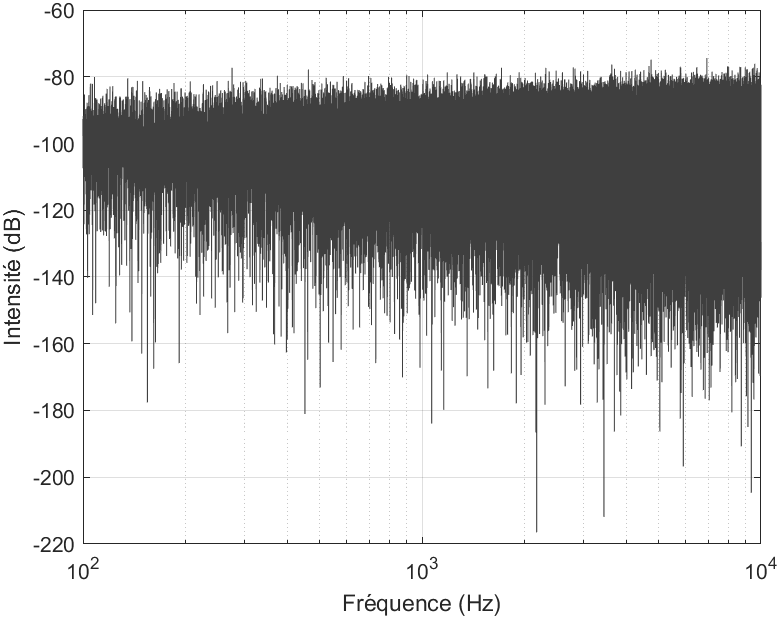
\includegraphics[scale=0.5]{img6.png}
        \caption{Espectro del ruido Blanco (espectro plano) generado en Matlab R2020a.}
    \end{figure}

    \item[-] \textbf{Le bruit rouge ou brownien} correspond dans une première approximation, dans les domaines qui utilisent des définitions précises, la terminologie « bruit rouge », « bruit brownien » ou « bruit brun » fait référence au son ayant une puissance sonore qui décroît de 6 dB par octave lorsque la fréquence augmente (densité proportionnelle à 1/f ) sur un intervalle de fréquence n'incluant pas de DC (Qui dans un sens général, n'inclut pas de composante constante, ou de valeur pour f=0). 

    % Imagen
    \begin{figure}[H]
        \centering
        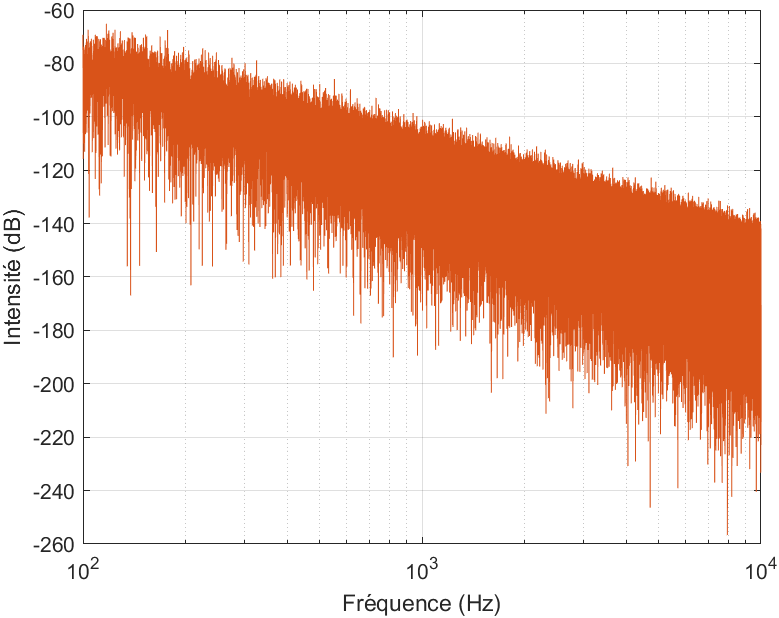
\includegraphics[scale=0.5]{img7.png}
        \caption{Espectro del ruido Café (-$6dB$/Octava) generado en Matlab R2020a.}
    \end{figure}

    D’un autre point de vue, dans les domaines qui utilisent des définitions plus approximatives, le « bruit rouge » correspond à tout son dont la densité de puissance diminue lorsque la fréquence augmente3. 

    Plus exactement Le bruit rouge, peut être obtenu en utilisant un algorithme simulant le mouvement brownien ou par intégration mathématique du bruit blanc.
    
    \item[-] \textbf{Le bruit rose} se caracteriza por su densidad espectral decreciente de –3$dB$/Octava. Su percepción se asemeja a escuchar sonidos de la naturaleza como lluvia constante.
    
    % Imagen
    \begin{figure}[H]
        \centering
        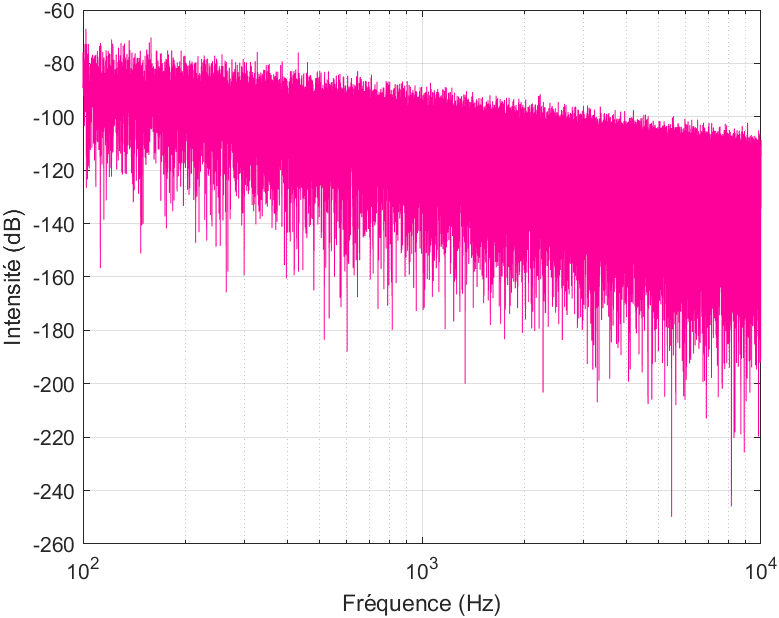
\includegraphics[scale=0.5]{img8.png}
        \caption{Espectro del ruido Rosa (-$3dB$/Octava) generado en Matlab R2020a.}
    \end{figure}

    \item[-] \textbf{Le bruit bleu} qui correspond à un bruit qui augmente sa puissance sonore de 3 dB par octave lorsque la fréquence augmente (densité proportionnelle à f), et ce jusqu’à une fréquence infinie. 

    Dans le domaine de l’informatique graphique, le terme « bruit bleu » est parfois utilisé d’une façon plus approximative pour décrire tout son de puissance sonore minimale à basse fréquence et ne présentant aucun pic lorsque la fréquence augmente (croissance constante). 

    Il est convenable de connaitre et différencier aussi le bruit rose des autres types de bruits coloré, dans la mesure que ce type de bruit fait partie de notre étude. Donc le bruit rose, ce type de bruit est caractérisé par une puissance égale sur des bandes proportionnelles en largeur. Une bande correspond en fait à un changement de fréquence (hausse ou baisse à exprimer en pourcentage de l’une des extrémités de l’intervalle). Par exemple, la puissance d’un bruit rose est la même sur les intervalles allant de 40 à 60 Hz et de 4000 à 6000 Hz car ces intervalles sont proportionnels (ils correspondent à une hausse de 50 pourcent de la fréquence). 

\end{itemize}
\hfill

Dans un deuxième temps, nous voyons l’existence d’une deuxième
famille de bruits que nous choisissant de nommé des bruits
industriels. En effet, comme son nom l’indique les bruits
industriels sont des perturbations sonores produits par l’industrie
ou par des effet industrie. Dans cette famille nous trouvons des
bruits tels que le bruit de route qui est un bruit normalisé. Il est
une référence pour le bruit des trafics routiers et ferroviaires.
Son spectre est enrichi en basses fréquences et appauvri dans les
aiguës par rapport à un bruit rose. Mais aussi nous trouvons des
bruits comme les suivants :
\hfill

\begin{itemize}

    \item[-] \textbf{Le bruit d’impact}: c’est le bruit transmis par une paroi mise en vibration par un choc (bruit de pas, déplacement de meubles, chute d’objet, enfoncement d’un clou dans un mur...).
    \item[-] \textbf{Le bruit aérien}: c’est le bruit propagé dans l’air (bruit de voix, bruit de télévision, bruit de circulation...). 
    \item[-] \textbf{Le bruit solidien}: c’est le bruit propagé dans les milieux solides comprenant (le bruit d’impact transmis par les éléments solides, le bruit d’équipement (chaufferie, ascenseurs, ...). 
    
\end{itemize}

\clearpage
\section{Méthodes}
Le but de ce projet est de implementer le filtrage dans les notes audios dans l'objectif d'attenuer le bruit present. Pour cela nous allons implementé le filtrage analogique avec une approximation de Butterworth, la méthode RNN et un autre qui reste définir.

\subsection{\textbf{Filtre de Butterworth}}

\subsection{\textbf{Filtre de Wiener}}
Le filtre de Wiener est une des meilleur filtres linaires de minimum carré. Il peut être utilisé pour prédire, estimer, interpoler, filtrer un signal et le bruit, entres autres. Pour créer ce type de filtre, il faut connaitre avoir une connaissance préalable du signal que le système aura comme entrée, c’est à dire le signal qui sera filtré. Le plus grand problème c’est que cette information est difficile à obtenir, c’est pour cela que les filtres adaptatifs sont très importants, parce qu’ils utilisent les données d’entrée pour pouvoir déterminer les données statistiques requis. En général, on a un signal $f(k)$, une réponse désiré $d(k)$ et un filtre linéaire de réponse impulsionnelle $h(k)$. Ce filtre est alimenté par $f(k)$ et produit une sortie $g(k)$. La différence entre le signal de sortie $g(k)$ et le signal désiré $d(k)$, est connue comme erreur d’estimation $e(k)$, la figure suivante illustre ce fait :

% Imagen

\begin{figure}[H]
 \centering
    \includegraphics[width=0.5\textwidth]{Wiener.png}
    \caption{Filtre de Wiener}
\end{figure}

L’objectif du filtre de Weiner est de déterminer la réponse impulsionnelle $h(k)$ dans le but de produit une erreur $e(k)$ le plus petit possible. Le critère utiliser pour réaliser cela est la minimalisation du valeur quadratique moyen de l’erreur.

Le filtre digital montrer dans l’image a un signal d’entre et produit un signal de sortie. Le filtre sera un filtre de Wiener si sa réponse impulsionnelle est choisie dans l’objectif de minimiser l’erreur quadratique moyen. L’erreur est définie comme la différence entre la sortie et la réponse désiré et est décrit par l’équation suivante :
\begin{center}
     $e_k=d_k-g_k$
\end{center}{}

Lorsque nous travaillons avec le filtre de Weiner, généralement la réponse désirée existe dans la forme théorique. Cependant, dans ce cas on travaille avec un réponse désiré connue. La réponse impulsionnelle du filtre de Weiner est obtenue 

Si nous appliquons le carré a l’équation de l’erreur, nous avons :

% ecuación
\begin{center}
    $e_k^2=d_k^2+g_k^2-2d_kg_k$
\end{center}{}
    

Et on sait que :

% ecuación
\begin{center}
     $g_k$ =$\displaystyle\sum_{l=0}^{\infty}f_{k-l} h_l $
\end{center}


Si on substitue dans l’équation de l’erreur, on a :

% ecuación
\begin{center}
    $e_k^2=d_k^2+$ $\displaystyle \sum_{l=-\infty}^{\infty}\displaystyle\sum_{m=-\infty}^{\infty}$$h_l h_\mu f_{k-l} f_{k-\mu}$ $- 2$  $\displaystyle\sum_{l= -\infty}^{\infty}f_{k-l} h_l d_k$
\end{center}

Si, on prend la valeur moyenne à chaque côté, on trouve une expression pour l’erreur quadratique moyenne 

% ecuación
\begin{center}
     $E[e_k^2]=E[d_k^2]+$ $\displaystyle \sum_{l=-\infty}^{\infty}\displaystyle\sum_{m=-\infty}^{\infty}$$h_l h_\mu E[f_{k-l} f_{k-\mu}]$ $- 2$  $\displaystyle\sum_{l= -\infty}^{\infty}h_l E[f_{k-l}  d_k]$
\end{center}
\begin{center}
        $= \phi_{dd} (0) + $ $\displaystyle \sum_{l=-\infty}^{\infty}\displaystyle\sum_{m=-\infty}^{\infty}$ $h_l h_\mu \phi_{ff} (l-\mu)$  $- 2$  $\displaystyle\sum_{l= -\infty}^{\infty} h_l \phi_{fd}(l)$
\end{center}

Avec $\phi_{dd}$ et $\phi_{ff}$ l’autocorrélation et $\phi_{fd}$ la corrélation croisée entre les signaux $f$ et $d$. Si on dérive en fonction de $h$ et on cherche la solution de l’équation lorsque celle-ci tend vers $0$, on a :

% ecuación
\begin{center}
     $\displaystyle\sum_{l= -\infty}^{\infty}$ $h_l^* \phi_{ff} (j-l)=\phi_{fd}(j)$
\end{center}

Cette équation est l’équation de Wiener-Holpf, qui peut être écrit de la façon suivante, grave au produit de convolution :

% ecuación
\begin{center}
     $h_l^* * \phi_{ff} (k) = \phi_{fd} (k)$
\end{center}
Et si on applique la transformé en $Z$ a chaque partie de l’équation, on a :

% ecuación
\begin{center}
     $H^*(z) \phi_{ff}(z)=\phi_{fd}(z)$  ó  $H^*(z)=\frac{\phi_{fd}(z)}{\phi_{ff}(z)}$
\end{center}

Avec la solution de Weiner, on pet trouver la fonction de transfert du filtre $H(z)$ a partie de la transformé en $Z$ de la fonction d’autocorrélation d’un signal d’entrée, de la corrélation croisée du signal d’entré et la réponse désirée. Si on remplace cette équation dans l’expression de l’erreur, on a la valeur minimal MSE :

% ecuación
\begin{center}
     $E(e_k^2)_{min}=\phi_{dd}(0)-$ $\displaystyle\sum_{l= -\infty}^{\infty}h_l^* \phi_{fd}(l)$
\end{center}


\subsection{\textbf{RNNbruit: Méthode hybride DSP/Deep Learning}}
La méthode RRNbruit est une méthode créé para Jean-Marc Valin de Mozilla Corporation. Il s’agit d’une méthode hybride pour atténuer le bruit, en thermes général elle fonction de la façon suivante : elle utilise le Deep Learning dans des cas où la réduction du bruit demande réglage ou une configuration minutieuse, alors que pour les cas qui ne le demande pas, la méthode emplois des procèdes d’élimination du bruit classiques. Pour mieux comprendre le fonctionnement de ce filtre, nous allons étudier plus attentivement les concepts qui ont un rôle important dans cette méthode, tels que réseau de neurones artificiels, Deep Learning et réseau de neurones récurrentes.
\hfill\\

\subsubsection{Réseau de neurones artificiels}
Pour pouvoir comprendre de quoi il s’agit un réseau de neurones, il est convenable de commencer par un élément de ce réseau : un neurone artificiel. Il existe plusieurs modèles de neurones artificiels, cependant, il suffit de de définir le plus bas niveau, le perceptron, et le modèle le plus utilise dans les industries modernes, le sigmoïde. 
\hfill\\

\paragraph{Perceptron}
Les perceptrons ont été développer entre les années 1950 et 1960 par le scientifique Frank Rosenblatt, inspirée du travail réalisé par Warren McCulloch et Walter Pitts en 1943. 

Un perceptron prend plusieurs entrée binaires (uniquement de $0$ et de $1$) $x_1, x_2, ...$ et produit une unique sortie binaire, par exemple : 

%imagen
 \begin{figure}[H]
 \centering
    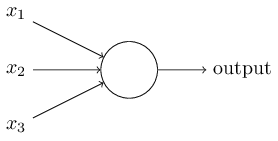
\includegraphics[scale=0.5]{img9.png}
    \caption{Ejemplo de la representación gráfica de un perceptrón.}
\end{figure}

Dans ce cas le perceptron a 3 entrées, amis en général il peut avoir une quantité arbitraire d’entrées, Rosenbatt propose une règle simple pour calculer la sortie. En effet, il introduit de poids $w_1, w_2, ...$ qui représentent des nombres réels illustrant l’importance de chaque entrée respectivement avec la sortie. La sortie de la neurone ($0$ ou $1$)  résulte de la somme pondérée des entrées, si cette somme est supérieure à une valeur limite, la sortie sera égale à $1$, mais si elle est inferieurs à cette valeur limite la sortie sera $0$. 

%ecuacion
\begin{equation}
    output =
    \begin{cases*}
      0 & if $\Sigma_j w_jx_j \leq $ threshold \\
      1 & if $\Sigma_j w_jx_j > $ threshold \\
    \end{cases*}
\end{equation}

La valeur limite est aussi un nombre réel. Il s’agit d’un paramètre du neurone. Pr notation, on simplifie la description précédant en considérant $w$ et $x$ comme des vecteurs des poids et des entrées, respectivement, donc la somme pondérée devient : 

%ecuacion
\begin{equation}
    w \cdot x \equiv \Sigma_j w_jx_j
\end{equation}

Finalement, on définit le biais noté b comme $b \equiv -$threshold, alors on a: 

%ecuacion
\begin{equation}
    output =
    \begin{cases*}
      0 & if $w \cdot x + b \leq 0$ \\
      1 & if $w \cdot x + b > 0$ \\
    \end{cases*}
\end{equation}

Il faut comprendre le biais comme un objet de mesure qui permet de déterminé à quel point il est facile de faire que la sortie du perceptron soit égale à $1$. En termes biologiques, le biais est une mesure qui permet de savoir à quel point il est facile de faire que le perceptron se déclenche ou s’active. 

Même si les perceptrons sont très utilisés pour modéliser une grande variété de problèmes, ils ont un grand désavantage. En effet, un petit changement dans le vecteur des biais ou dans celui des poids, peut entrer un grand changent dans la sortie, ce qui peut être problématique, même dans le cas d’un algorithme de bas niveau d’apprentissage.
\hfill\\

\paragraph{Neurones Sigmoïdes}
Elles se représentent de la même façon que les perceptrons : 

%imagen
 \begin{figure}[H]
 \centering
    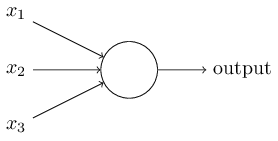
\includegraphics[scale=0.5]{img9.png}
    \caption{Ejemplo de la representación gráfica de un sigmoïde.}
\end{figure}

Elles ont un nombre arbitraire d’entrées $x_1, x_2, ...$, mais les valeurs des entrées prennent de valeurs comprises entre 0 et 1. Elles possèdent aussi un poids pour chaque entrée, $w1, w2, ...$, et un biais $b$. Dans ce cas, les sorties ne sont pas de valeurs de $0$ ou $1$, mais une fonction $g(w\cdot x+b)$, où g est appelé la fonction sigmoïde ou en général, fonction d’activation, et est définie par : 

%ecuacion
\begin{equation}
    g(z)=\dfrac{1}{1+e^-z}
\end{equation}

Où $z=w\cdot x+b$. Grafiquement est definie par:

%imagen
 \begin{figure}[H]
 \centering
    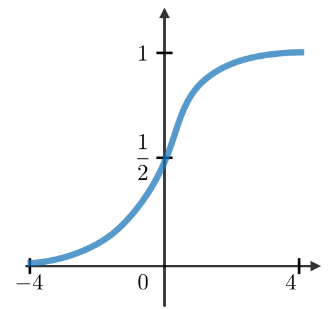
\includegraphics[scale=0.5]{img10.png}
\end{figure}

Dans ce cas, on observe que la sortie prend des valeurs entre $0$ et $1$, ceux qui revient à dire que la sortie peut prendre une infinité de valeurs. Usuellement, lorsqu’on emplois des sigmoïdes, l’intervalle est devisé en partitions et en fonction de la valeur obtenue, on fait une interprétation particulière de la sortie. Par exemple, en traitement d’image si on veut savoir si l’image d’entrée possède le numéro $9$, on pourrait employer une cote de $0.5$.  


\paragraph{Autres modèles de neurones utilisés dans le modèle}
La méthode RNNbruit emploie des réseaux de neurones avec de neurones sigmoïdes mais il peut employer deux autres modèles de neurones : $Tanh$ et $RELU$. Le comportement et la description de ces modèles est exactement le même, avec un changement de la fonction d’activation $g$. 

%imagen
 \begin{figure}[H]
 \centering
    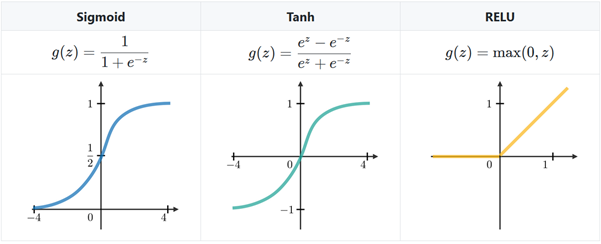
\includegraphics[scale=0.7]{img11.png}
\end{figure}


\subsubsection{Notation dans l’architecture des réseaux neuronales}
Les entrées sont encerclées et symbolisés : 

%imagen
 \begin{figure}[H]
 \centering
    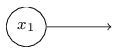
\includegraphics[scale=0.5]{img12.png}
\end{figure}

Considérons un réseaux neuronal arbitraire comme celui-ci-dessous : 

%imagen
 \begin{figure}[H]
 \centering
    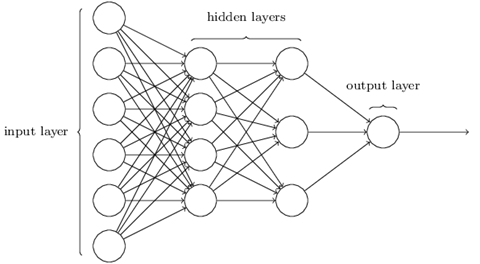
\includegraphics[scale=0.7]{img13.png}
\end{figure}


La colonne de gauche qui contient toutes les entrées est connue comme “couche d’entrée” (input layer en anglais). La colonne de droite qui contient toutes les sorties est connue comme “couche de sortie” (output layer en anglais). Les autres colonnes qui contiennent les neurones sont connues comme “couches cachés” (hidden layers en anglais). Dans le cas de l’image ci-dessus, on a un réseau neuronal avec 6 entrées (input features en anglais), 2 couches cachés et une sortie.  Il est important de remarquer que ce type de réseau neuronal, qui est composé d’une couche d’entrées, 2 couches cachées et une couche de sortie, est connue sous le nom de réseau neuronal pré-alimenté.
\hfill\\

\subsubsection{Réseau de neurones récurrents (Recurrent Neural Networks, RNN)}

Les réseaux de neurones récurrents sont un autre type de réseau de neurones. Il se caractérisent par le fait que la sortie donnée par une neurone est la sortie générale du réseau et au même temps, cette sortie est l’entrée pour le neurone suivante, comme l'ilustre l'image ci-dessous : 

%imagen
 \begin{figure}[H]
 \centering
    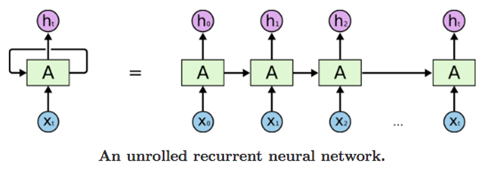
\includegraphics[scale=0.5]{img14.png}
\end{figure}


Le réseau de neurones récurrent est symbolisé comme le réseau de gauche avec une boucle de retro alimentation, cependant, il est plus de comprendre son fonctionnement en la “déroulant” (unroll en anglais) comme nous pouvons voire dans le réseau de neurones équivalent de droite. Dans ce cas, les neurones sont représentés par des rectangles en vert et la lettre $A$, les entrées sont représentées par des cercles bleus et la lettre $X$ avec un indice, et les sorties son représenté par des cercles violets et la lettre $h$ avec un indice. Il faut remarquer que dans ce cas la couche d’entrée correspond à la rangée qui contiens toutes les entrées en bleus, la couche de sortie correspond à la rangé supérieure qui contiens toutes les sorties en violet et la couche restante est la seule couche cachée. 

On observe que le neurone $A$, dans un premier temps, a comme entrée $X_0$. Elle réalise une fonction en fonction du type de neurone duquel elle fait partie et produit comme sortie la première sortie du réseau $h_0$.  Cette neurone fiat une retro alimentation avec la sortie qu’elle produit lorsque l’entrée est $X_1$ et ainsi de suite. Dans d’autres réseaux de neurones, les entrées sont indépendantes les unes avec les autres, mais dans le cas des réseaux de neurones récurrents toutes les entrées sont reliées avec les autres. 

C’est-à-dire qu'un réseau de neurones récurrents, contrairement à un réseau de neurones pré alimenté, peut utiliser l’état internet des neurones (mémoire) pour traiter des séquences d’entrées. Ceci explique pourquoi elles peuvent être utiliser pour des travaux comme la reconnaissance d’écriture ou vocale. 

La formule qui décret la sortie d’un réseau de neurones récurrent est la suivante :

\begin{equation}
    h_t = g(w_{t-1}h_{t-1} + w_tX_t) 
\end{equation}


Où g est la fonction d’activation du neurone.  


\clearpage % salto de página
\section{Résultats et comparaison des méthodes}
Los métodos fueron implementados de forma cuantitativa y cualitativa. Para ambos casos se utilizó el software Matlab R2020a en el SO Microsoft Windows 10 Home Single Language (v. 10.0.19041). Para los casos de implementación se generó ruido blanco, rosa y café utilizando el software Audacity 2.4.2. Luego en Matlab se tomó el audio original y se crearon 3 audios adicionales al mezclar el audio original con 30\% de ruido blanco, 30\% de ruido rosa y 30\% de ruido café, respectivamente.

\subsection{Résultats quantitatifs}
En la tabla \ref{table:t1} se muestra el porcentaje de ruido
resultante al aplicarle 30\% de ruido blanco al audio original y
filtrarlo con cada uno de los métodos.  
\begin{table}[hbt!]
    \centering
    \begin{tabular}{ l  c }
    \textbf{Méthodes} & \textbf{Blanc (30\%)} \\
    \hline
    Sans méthode & 80.658 \\
    Wienner & 73.621 \\
    Butter T & 10 \\
    RNNbruit & 9.9668 \\
    \end{tabular}
    \caption{Résultats des méthodes pour 30\% du bruit blanc}
    \label{table:t1}
\end{table}
\hfill \\
En la tabla \ref{table:t2} se muestra el porcentaje de ruido resultante al aplicarle 30\% de ruido rosa al audio original y filtrarlo con cada uno de los métodos.  
\begin{table}[hbt!]
    \centering
    \begin{tabular}{ l  c }
    \textbf{Méthodes} & \textbf{Rose (30\%)} \\
    \hline
    Sans méthode & 39.442 \\
    Wienner & 65.359 \\
    Butter T & 35 \\
    RNNbruit & 11.493 \\
    \end{tabular}
    \caption{Résultats des méthodes pour 30\% du bruit rose}
    \label{table:t2}
\end{table}
\hfill \\
En la tabla \ref{table:t2} se muestra el porcentaje de ruido resultante al aplicarle 30\% de ruido café al audio original y filtrarlo con cada uno de los métodos. 
\begin{table}[hbt!]
    \centering
    \begin{tabular}{ l  c }
    \textbf{Méthodes} & \textbf{Marron (30\%)} \\
    \hline
    Sans méthode & 53.969 \\
    Wienner & 62.248 \\
    Butter T & 35 \\
    RNNbruit & 7.7496 \\
    \end{tabular}
    \caption{Résultats des méthodes pour 30\% du bruit Marron}
    \label{table:t3}
\end{table}
\hfill \\
Premièrement, en étudiant les résultats obtenus par l'implémentation du filtre passe-bas avec une approximation de Butter Worth, nous confirmant les hypothèses théoriques vues précédemment. En effet, compte tenu que l’approximation de Butter Worth permet d’avoir une précision en amplitude. Cette précision est centre sur des bases fréquences. Nous voyons cela évidence dans le filtrage des bruits ajouter à notre signal. Lorsque nous ajoutons du bruit blanc et nous filtrons le signal résultant, nous constatons une diminution du pourcentage du bruit présent dans le signal. Alors que lorsque nous effectuons le même procédé pour le bruit rose et le bruit marron, le pourcentage de bruit ne change pas. Donc cette méthode avec cette approximation particulière est bien plus convenable pour filtrer le bruit blanc présent dans les enregistrements audios.

Dans un deuxième temps, le cas de la méthode hybride du RNNbruit, nous observons que cette méthode est belle et bien convenable pour les différents types de bruit additionnés. En effet, nous constatons une atténuation du bruit considérable dans chacun des cas. De plus, nous remarquons que cette méthode ne gêne pas la transmission du signal sonore, en d'autre thermes cette méthode lise et "purifie" le signal orignal. Nous pouvons expliquer ce comportement par la nature adaptative de la méthode, dû au fait de l'implémentation de réseau de neurones récurrents pour faire face au bruit non harmonique. Cependant, la partie traditionnelle de cette méthode dite hybride se charge du bruit harmonique comme nous l'avant vue précédemment dans la partie théorique.

Finalement, lorsque nous analysons les résultats obtenus en utilisant le filtre adaptatif de Weiner, nous apercevons que cette méthode de filtrage numérique a des meilleurs résultats sur du bruit blanc. Or, en effectuant une analyse auditive, nous pourrions penser que ce filtrage est bien plus efficace avec le bruit marron ou le bruit rose, nous pouvions affirmer théoriquement que ‘est avec le bruit blanc qu’il est plus efficace. En effet, en employant cette méthode nous introduisons des nouveaux types de bruits que nous ne considérerons pas dans notre analyse. Par exemple, dans le filtrage de l’enregistrement audio avec du bruit marron, nous pouvons avoir l’impression que le résultat est nettement plus compressible qu’avec du bruit blanc. Cependant, en regardant les résultats de l’analyse nous nous rends compte que l’audio résultant a perdu de l’intensité sonores, c’est-à-dire que l’amplitude de son gain en fréquence a considérablement diminuer. Cette méthode, théoriquement parlant, nous est convenable dans la mesure ou elle permet un filtrage du bruit blanc, mais elle rencontre ses limites avec les 2 autres types de bruit étudiés.


\subsection{Résultats qualitatifs}
\hfill
En la tabla \ref{table:t4} se muestra la calificación que se le dio a cada uno de los métodos para el audio original mezclado con 30\% de ruido blanco.
\begin{table}[hbt!]
    \centering
    \begin{tabular}{ l  c }
    \textbf{Méthodes} & \textbf{Blanc (30\%)} \\
    \hline
    Sans méthode &  \\
    Wienner &  \\
    Butter T &  \\
    RNNbruit &  \\
    \end{tabular}
    \caption{Qualification des méthodes pour 30\% du bruit blanc}
    \label{table:t4}
\end{table}
\hfill \\
En la tabla \ref{table:t5} se muestra la calificación que se le dio a cada uno de los métodos para el audio original mezclado con 30\% de ruido rosa.  
\begin{table}[hbt!]
    \centering
    \begin{tabular}{ l  c }
    \textbf{Méthodes} & \textbf{Rose (30\%)} \\
    \hline
    Sans méthode &  \\
    Wienner &  \\
    Butter T &  \\
    RNNbruit &  \\
    \end{tabular}
    \caption{Qualification des méthodes pour 30\% du bruit rose}
    \label{table:t5}
\end{table}
\hfill \\
En la tabla \ref{table:t6} se muestra la calificación que se le dio a cada uno de los métodos para el audio original mezclado con 30\% de ruido café.
\begin{table}[hbt!]
    \centering
    \begin{tabular}{ l  c }
    \textbf{Méthodes} & \textbf{Marron (30\%)} \\
    \hline
    Sans méthode &  \\
    Wienner &  \\
    Butter T &  \\
    RNNbruit &  \\
    \end{tabular}
    \caption{Qualification des méthodes pour 30\% du bruit Marron}
    \label{table:t6}
\end{table}
\hfill \\


\clearpage

\section{Méthodes modifiées}
En esta sección se realizan las descripciones e implementaciones de las modificaciones propuestas para cada uno de los métodos.

\subsection{\textbf{Butterworth modifiée}}

\subsection{\textbf{Wiener modifiée}}

\subsection{\textbf{RNNbruit modifiée}}


\end{document}
